\documentclass[12pt, letterpaper, titlepage]{article}

\usepackage{amsmath, amsfonts}
\usepackage{booktabs}
\usepackage{amsthm}
\usepackage{graphicx}
\usepackage[margin=1in]{geometry}
\usepackage{hyperref}
\usepackage{cleveref}
\hypersetup{colorlinks = true, linkcolor = blue, citecolor=blue, urlcolor = blue}
\usepackage{natbib}
\usepackage{float}
\usepackage{setspace}
\usepackage{pdfpages}
\usepackage[pagewise]{lineno}
\usepackage{mwe}
\usepackage{comment}
%\linenumbers*[1]
% %% patches to make lineno work better with amsmath
\newcommand*\patchAmsMathEnvironmentForLineno[1]{%
 \expandafter\let\csname old#1\expandafter\endcsname\csname #1\endcsname
 \expandafter\let\csname oldend#1\expandafter\endcsname\csname end#1\endcsname
 \renewenvironment{#1}%
 {\linenomath\csname old#1\endcsname}%
 {\csname oldend#1\endcsname\endlinenomath}}%
\newcommand*\patchBothAmsMathEnvironmentsForLineno[1]{%
 \patchAmsMathEnvironmentForLineno{#1}%
 \patchAmsMathEnvironmentForLineno{#1*}}%

\AtBeginDocument{%
 \patchBothAmsMathEnvironmentsForLineno{equation}%
 \patchBothAmsMathEnvironmentsForLineno{align}%
 \patchBothAmsMathEnvironmentsForLineno{flalign}%
 \patchBothAmsMathEnvironmentsForLineno{alignat}%
 \patchBothAmsMathEnvironmentsForLineno{gather}%
 \patchBothAmsMathEnvironmentsForLineno{multline}%
}

% control floats
\renewcommand\floatpagefraction{.9}
\renewcommand\topfraction{.9}
\renewcommand\bottomfraction{.9}
\renewcommand\textfraction{.1}
\setcounter{totalnumber}{50}
\setcounter{topnumber}{50}
\setcounter{bottomnumber}{50}

\newcommand{\jy}[1]{\textcolor{blue}{JY: #1}}
\newcommand{\eds}[1]{\textcolor{red}{EDS: (#1)}}
\newcommand{\of}[1]{\textcolor{violet}{OF: #1}}


\title{On Devon Allen's Disqualification at the 2022 Track and Field World
Championship} 

\author{Owen Fiore\\
%   \href{mailto:owen.fiore@uconn.edu}
% {\nolinkurl{owen.fiore@uconn.edu}}\\
  Elizabeth Schifano\\
  Jun Yan\\[1ex]
  Department of Statistics, University of Connecticut\\
}
\date{}

\begin{document}
\maketitle

%Abstract should be 200 words
%Devon Allen was disqualified in 2022... discussions about dq, talk methods and 
%models, venue effect, and conclusion
\begin{abstract}
Devon Allen was disqualified in the Men's 110 meter hurdle final of the 2022
World Track and Field Championships after registering a reaction time of 0.099 
seconds, 0.001 seconds faster than what is allowed. Following the games, 
bloggers on the running website LetsRun %scrutinized the results %and performed 
%non-statistical analysis of the data. They found 
concluded that the reaction time data from the 2022 World Championships 
seemed to be generally faster compared to the other datasets they looked at, but 
they did not perform any formal %meaningful 
statistical analyses. This paper questions the reaction time 
disqualification barrier, which is currently 0.1 seconds, to determine whether 
this is a reasonable threshold. We employ a generalized linear mixed model 
(GLMM) with a random %effect term which will be referred to as the 
venue effect in order to %try and 
model the data. Additionally, we employ a signed-rank test for clustered data to 
compare reaction times for the same athletes at different competitions. This 
matter needs to be addressed because %Devon Allen's 
disqualification based on allowable reaction time 
%could be a 
%problem that could 
will continue to be an issue in future world championships.

\jy{Avoid references in abstract.}

  
\jy{This is only the background. An abstract also needs to summarize the 
contributions.}
%\bigskip
\eds{removed Devon Allen from keywords because his name is already in title
and replaced with others}

\noindent\sc{Keywords}:
False Start, Hurdles, Reaction Time, Seiko, 2022 World Track and Field Championships 

\end{abstract}

\doublespace

\jy{The bib file needs quality control. Practice my writing tips in the
  stat-wriging notes: chapter 2 on latex/bibtex.}

\jy{Go over the reference section to see what need to be changed in the bib source}

\jy{Turn on column numbers in your editor to keep line width under 80.}

\section{Introduction}
\label{sec:intro}


\jy{Not a good opening. Could start by telling the story, recapping the major
  events and discussions on the internet. Then dig into the relevant
  literature. Finally outline the contributions of this work.
}


\jy{use the following structure and flow:
  1) A paragraph to tell the story;
  2) A paragraph on informal statistical analyses on the internet/social media;
  3) A paragraph on scholarly articles on reaction time in the literature;
  4) A paragraph on what's new: methods; results.
  5) A paragraph of roadmap.}


%1)
Devon Allen, an alumnus of the University of Oregon in 
Eugene, Oregon, was
expected to be a contender for the 2022 World Track and Field Championships 110 
meter hurdle.  After running the event in 12.84 seconds in early June 2022 
(only 0.04 seconds away from the world record \citep{wa2022preview}) and coming 
in third in the event at the United States Track and Field 
Championships also in Eugene at the end of June, Allen was poised to 
compete in the 2022 World Track and Field Championships again in Eugene in August.
%After coming in third in the 110 meter hurdles at the United States Track and 
%Field Championships also in Eugene at the end of June, Allen was poised to 
%compete in the 2022 World Track and Field Championships also 
%located at Eugene in August.
%two months later. 
At the World Championships, Allen made it through the 
heats and semifinals to reach the finals while posting reaction times of 0.123
in the heats \eds{if more than one heat, include all of them or the average;
if only one heat, change to singular form}
\of{There are roughly 5 heats, but each athlete only competes in one heat} 
and 0.101 in the semifinal.  
%Allen, who attended the University of Oregon also in Eugene, 
%(the location of US World Championship 
%\eds{US World? remove World?} and the World Championship) 
%was
%considered to be a favorite for the 110 meter hurdle after running 12.84 seconds
%in early June; only 0.04 seconds away from the world record \citep{wa2022preview}.
%Thus 
His disqualification by reacting in 0.099 seconds instead of 0.1 was met
with shock from both Allen and fans alike.  NBC, who was broadcasting the
championships in the United States, later uploaded a video to their YouTube
channel that showed the disqualification; it can be found here:
\url{https://www.youtube.com/watch?v=D6NXTMo-1yM}. The crowd erupted with jeers 
when they found out that Allen was disqualified, angry at the result.  Had Allen 
reacted just 0.001 seconds slower he would have been allowed to compete and been 
spared waiting another two years until the next World Track and Field Championship.

\eds{final two sentence seems out of place here; consider moving elsewhere?}
\of{Moved to the end of paragraph 4 of introduction}

%2)
Allen's disqualification has been discussed extensively in online communities
such as \url{www.LetsRun.com}, a website that is part message board and part
news. The message board,
which functions similarly to Reddit is very active during important running
events, including during the finals of major events such as
the Olympics and the World Track and Field Championships.  However, it is the
news section of the website that generated articles such as \citet{johnson2022was}
and \citet{johnson2022data} from  Robert Johnson, who created and runs 
the LetsRun website.  He argued that there was an error
with the timing equipment at the 2022 Track and Field World Championship and
cited graphs, simple statistics such as median reaction time, and compared the 
reaction times at the 2022 World Track and Field Championship to other competitions
such as the USA Track and Field Championships and other World Championships.
However, their analysis lacked formal analysis. The alleged 99.95\% chance Allen
was wrong came from that the lowest average reaction time for the men's 100 meter,
men's 110 meter hurdle, and women's 100 meters from 2003 to 2022 all occurred at
the 2022 World Championships and Johnson claimed that the probability of this
happening was $\frac{1}{13} \cdot \frac{1}{13} \cdot \frac{1}{13} = 0.05\%$
\citep{johnson2022was}.
\eds{compared the reaction times at the 2022 World Track and Field  Championship 
to what? Also restate here that no formal statistical analyses have been done.}
\of{Cleaned this up a little but still a little messy.}

%3)
%The International Association of Athletics Federations (also referred to
%as IAAF or World Athletics), which is the governing board for international running
%competitions, commissioned a study in 2009 regarding the reaction time 
%barrier and whether the threshold should be lowered. 
%The paper analyzed sprinters reaction times and the biological processes 
%that went into reacting to the starting gun and concluded 
%that athletes can react in as low as 0.08 seconds.  
%One study by Pain looked at
Reaction time in sprint and hurdle events has been studied by many authors.
\citet{pain2007sprint} examined
reaction times for nine male athletes.  The
fastest athlete of the nine had, on average (even with their two fastest times 
removed), a reaction time of 0.087 seconds and a standard deviation of 0.004
seconds.  Two other athletes were able to react similarly when under certain
muscular tightening conditions \citep{pain2007sprint}. 
In a study commissioned by International Association of Athletics Federations 
(IAAF), \citet{komi2009iaaf} recommended that the disqualification 
barrier be decreased to allow sprinters to
react faster, and suggested 0.08 or 0.085 seconds as possible new thresholds.
Additionally, it was recommended to IAAF that high speed cameras be used to
change the reaction time criteria from pushing off on the block to body
movement. This could provide a more accurate representation of reaction time, 
and thus the possibility of a false disqualification would be lowered.
The possibility of using a video-based medium has been proved to be a reliable
measure of reaction time \citep{mudric2015evaluation}.


\jy{Could be condensed}
\citet{pilianidis2012start} found
significant differences between reaction times at several world championships
between 1997 and 2009 for the men's 110 meter hurdles.  Another important
conclusion was that reaction times did not decrease over the twelve years
covered by the research in the study \citep{pilianidis2012start}. This contradicts
what was found in a 2021 study that concluded the year of competition has a
significant effect on reaction times \citep{zhang2021correlation}.  Their
analysis looked at data from the 2011-2019 World Championships across multiple
sprint events and concluded that from 2011 to 2019, reaction times got
faster. However, not all studies have been in favor of a decrease in the
reaction time barrier. \citet*{brosnan2017effects} argue for increasing 
the reaction time barrier to 0.115 seconds, and cited evidence from European 
Championships and World Championships in their article.  A study looking 
at the 2008 Olympics likewise supported the conclusion that athletes could not
react in as little as 0.1 seconds \citep{lipps2011implications}.  Another study
concluded that visual reaction times to the starting gun may be faster by 0.007
seconds than the IAAF method, which is from force on block starts 
\citep{holmes2018method}.  While this may seem trivial, Allen was disqualified
only by 0.001 seconds. It is also worth noting that one study looking at data 
from various IAAF meets found that the fastest reaction times for men were found
between the ages of 26 and 29 \citep{tonnessen2013reaction}.  This is notable 
because Allen was 27 years old at the 2022 Track and Field World Championship 
and in his physical peak.

%This will
%be important when considering the results in section \ref{sec:Results}.

Despite their study, IAAF has not changed the reaction barrier since it was
implemented at the 1999 World Track and Field Championships.  It is confusing
as to why IAAF would commission a study only to disregard the results and not
make the necessary changes.  It is unknown how many athletes since 2009 could
have potentially benefited from this, but it is probable that there are others
besides Allen who were disqualified.
%Reaction time barrier has been examined before: cite reviews
%Then go into specifics and talk about people who wanted to change barrier
%General reviews are important
%People have studied the biological processes, cite a few references
%How barrier is picked by regulator
%Read abstract and into and summarize into about one sentence what each paper contributes
%1 and 2 can be merged but 3 need to stand alone

%4)
\jy{language needs to be formalized and condensed.}
The objective to this paper is to analyze the reaction times at the 2022
World Track and Field Championship to check for any abnormalities, and we approach
this two different ways.  First we try to model the data, which is
the reaction times of every non-disqualification since the 1999 World Championships. 
The model we use is a gamma linear mixed-effects model with a random effect
accounting for the venue (or year) effect. 
Then we compare reaction times for athletes who have competed
at additional competitions to the 2022 World Track and Field Championship.  By
comparing the same athlete across multiple competitions we are able to see if the
2022 data differed significantly from other competitions.
Our investigation into reaction times is important because reaction times have
been shown to affect the overall time of the race \citep{delalija2008reaction}.
Thus, faster reaction times lead to faster overall times; which is the goal of
every sprinter who steps onto the track.
%\eds{I recommend moving the rest of this paragraph to Section 2.2 as I don't
%think it is critical for readers to know all the details here.}
%First we can compare the reaction times of athletes who
%competed at the World Track and Field Championship in both 2019 and 2022, and 
%second we can compare how athletes performed at the 2022 championship relative 
%to their national/qualifiers meet. In order to reduce any chances
%of athletes improving reaction time, we can also look at data from qualifying meets.
%Almost every athlete had to qualify by proving they are elite at the national level, 
%usually by coming in at least fourth. Thus, data was compiled on athletes who competed
%at the 2022 World Track and Field Championships on what these athletes also ran 
%at their country's national championship. If there was any argument that athletes
%have improved their reaction time from 2019 to 2022, it should now be considered
%nearly null, as the national competitions took place between June and July 2022 
%and the World Championships were in August. The equipment used to measure reaction
%time cannot be guaranteed to be the same from national to international
%competition, but the time span between meets has been reduced considerably.


The rest of this paper is organized as follows. Section~\ref{sec:Data} describes 
how data was collected and begins to detail the generalized linear mixed-effect 
(GLMM) model that is further developed in Section~\ref{sec:Methods}. The 
signed-rank test that analyzes reaction times for the same athletes is
also described in Section~\ref{sec:Methods}.  Section~\ref{sec:Results}
 provides the results of the two analyses and ends 
by questioning the reaction time barrier.  Lastly, Section~\ref{sec:Discussion}
discusses the impact and limitations of the paper.
\eds{capitalize first letter when referring to a numbered section, table, figure, 
etc. ``Section 4 provides...'' vs. ``The next section provides...''}


\section{Data} \label{sec:Data}

There are two types of data that are explored throughout this paper: data from
1999-2022 for every world championship, and data from athletes who competed
the 2022 World Championships and another competition (either 2019 World 
Championship or a 2022 national competition held within two months of the  
2022 World Championships). The first data set is used for the GLMM portion
of the paper, while the second data set is used for the rank-based comparisons.

\subsection{World Championship}


\begin{figure}[tbp]
  \centering
  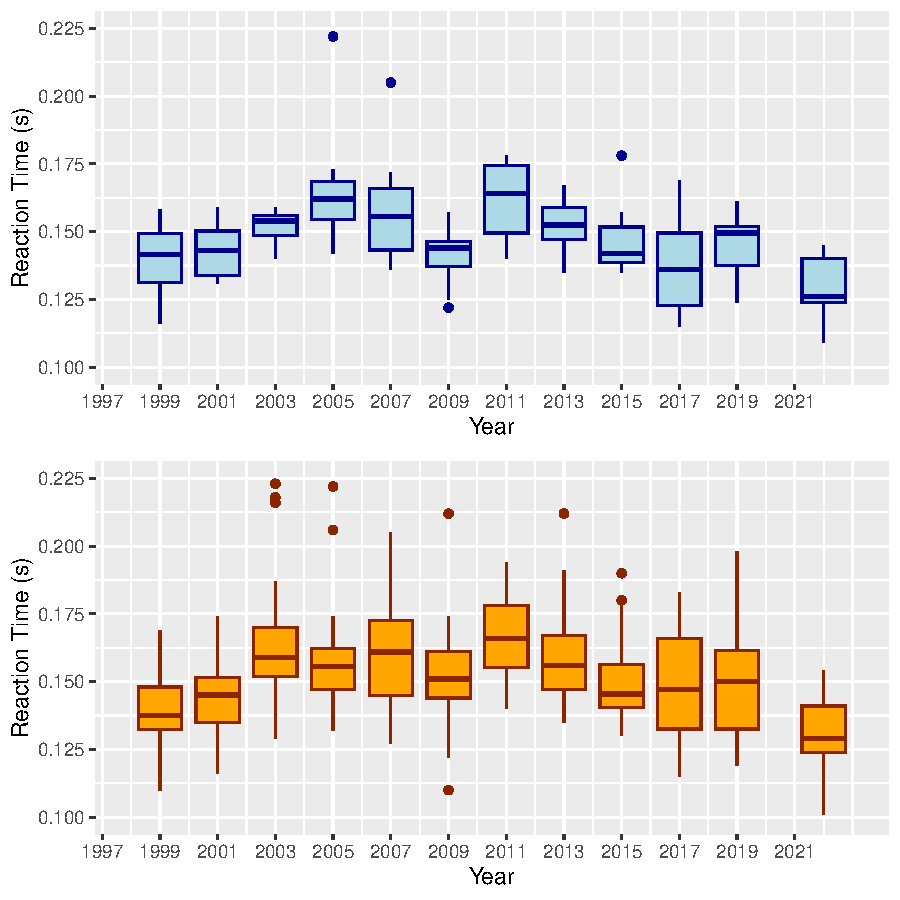
\includegraphics{Finals_Pooled_Boxplot}
  \caption{The reaction times from 2019 to 2022 for the men's final (top) and
  the men's semifinals and finals (bottom).}
  \label{fig:Boxplots}
\end{figure}


Data was taken from the World Athletics and covers the men's 110 meter hurdles 
and the women's 100 meter hurdles from 1999 to 2022.  The variable of prediction 
interest is reaction time, and the predicting variables are year, stage of 
competition (heats, semifinal, final), total time, and gender.  
The data can be found in the appendix~\ref{sec:Appendix}. Factors such as name, 
country, and identification number were not considered important for the 
purposes of this research besides the times for Devon Allen and the other 
United States athletes mentioned above.  The variable ``Stage"
refers to whether the observation occurred during the ``heats" (Preliminary round) which
is denoted by ``H" in the data, ``S" for ``semifinals" (Of which there are either 2 or 3 
heats each year), and ``F" for finals. The variable ``Gender" has levels ``M" and ``F" 
which stand for ``male" and ``female" respectively.  The variable ``Batch" takes a 
numerical value and every heat of every round from 1999 to 2022 was assigned it's
own number.  This was added because of suspected issues that reaction time may be
correlated with other runners reacting quickly (one runner reacting quickly may
result in other runners reacting quickly).  There is no statistical significance to
how the batches were labeled, they were ordered chronologically by meet but
reverse chronologically by year (Batch 1 is a preliminary Heat of 2022 and Batch
111 corresponds to the 1999 finals). Included are
box plots of the reaction times of the men's finals and the men's semifinals and
finals pooled together.  We will refer to the latter as the ``pooled data"
throughout the paper.  The heats or preliminary rounds were not studied because
athletes react faster as the competition progresses.  Athletes react faster in
the finals than the semifinals which are faster than the heats 
\citep{zhang2021correlation}.  If we want to determine if Allen's reaction time
is reasonable, then we thus need to look at the men's final data, with the men's
pooled data being included in order to increase the sample size.  In 2022, there
were only five data points due to two disqualifications and one athlete who 
qualified but did not compete.
The data that looked at in the paper is best visualized using a box plot as show 
in Figure~\ref{fig:Boxplots}.  It is clear that the 2022 box plot for both the
men's finals and semifinals data is lower (indicating a faster reaction time)
than in previous years.  The median for the men's pooled data in 2022 was 0.129
and the median for the men's final data in 2022 was 0.126.  For comparison,
Brosnan found reaction times of 0.156 seconds for men when looking at data from
1999 to 2014 \citep{brosnan2017effects}.


Something that is extremely important to note in the data is the inconsistency 
of World Athletics in terms of how they penalize false starts.  From 2007--2009,
the IAAF (the former name for World Athletics, and the governing body for the 
World Track and Field Champions) instituted a rule change that allowed one 
warning false start before a sprinter was disqualified \citep{iaaf2009falsestart}  This 
essentially gave sprinters a second chance and reduced the penalty for a false 
start.  There were 18 male and 7 female false starts at the 2007 World 
Championships, 18 male and 7 female starts at the 2009 World Championships. 
Starting in 2011, the rule was scrapped, and the old policy which automatically 
disqualifies runners who false start was reinstituted.  The effect? At the 2011 
World Championship there were 6 male disqualifications and 4 female 
disqualifications \citep{iaaf2009falsestart}. By returning to the harsher policy and 
cracking down on false starts, World Athletics had reduced the number of 
false starts by two thirds. One study that looked at different false start
rules that IAAF has imposed from 1997 to 2009 and found that the reaction 
times when there was less leniency improved by a statistically significant amount
\citep{haugen2013effect}. This was desirable for World Athletics as false starts can 
make already long track meets more tedious, both for athletes and viewers watching the 
television broadcast.  Since 2011, IAAF has instituted the one false start rule
\citep{iaaf2009falsestart}.  However, we chose not to include women's data in this
paper due to the numerous papers citing difference in reaction times in men and
women's reaction times: \citep{lipps2011implications, babicc2009reaction,
panoutsakopoulos2020gender}


\subsection{Beyond World Championship}
This section was motivated from a qualitative analysis that started by looking
at how United States athletes reacted at the 2022 United States Track and Field
Championships. From June 23-26 2022, USA held its Track
and Field Championship to decide who to send to the World Championships at Hayward 
Field, the exact same venue as used for the World Track and Field Championship a month 
later.  Thus, a baseline is able to be established for the four USA athletes who 
competed in at least one round of both events: Trey Cunningham, Daniel Roberts, 
Grant Holloway, and Devon Allen. Every athlete reacted faster in all the World 
Track and Field Championship races compared to the USA Track and Field 
Championship races. Devon Allen raced three times at the USA Track and
Field Championship and three times at the World Track and Field  Championship. 
His reaction times were significantly faster in the World Track and
Field Championship compared to the USA Track and Field Championship as were his
teammates.  This comparison suggests that the timing system used between the two
meets may have been meaningfully different to the point where Devon Allen was
disqualified more because of faulty equipment rather than because he reacted
too quickly.  Table~\ref{fig:USAvsWorld} highlights the difference in reaction times for
Devon Allen, Trey Cunningham, Grant Holloway, and Daniel Roberts. ``USA" denotes
the USA Track and Field Championships, ``World" denotes the World Track and Field
Championships,   All numbers listed in the table are the reaction
time for the respective athletes in seconds. 

\begin{table}
\begin{center}
  \caption{Reaction times for four United States Athletes at the 2022 USA Track
  and Field World Championships and the 2022 World Track and Field Championship.
  ``N/A" was used for any athlete that did not compete and thus did not register 
  a reaction time.}
  \begin{tabular}{c c c c c c c} 
   \toprule
   Athlete & USA H & USA S & USA F & World H & World S & World F \\ [0.5ex] 
   \midrule
   Devon Allen & 0.201 & 0.153 & 0.160 & 0.123 & 0.101 & 0.099 \\ 
   Trey Cunningham & 0.186 & 0.185 & 0.182 & 0.115 & 0.120 & 0.109 \\
   Grant Holloway & 0.192 & 0.190 & N/A & 0.147 & 0.128 & 0.124 \\
   Daniel Roberts & 0.181 & 0.200 & 0.183 & 0.179 & N/A & N/A \\ [0.5ex]
   \bottomrule
  \end{tabular}
  \label{fig:USAvsWorld}
  
  \end{center}
\end{table}

\jy{You have two such datasets in the analysis. Use one paragraph for each.}
\of{Split it into 2 sections, do you still want me to do something else?}

\eds{unless target journal has specified otherwise, Table captions should go
above the table. (Figure captions go below the figure)}
\of{Moved table caption to be above}


This dataset is quite small to perform any formal statistical analysis on, but
the data was expanded to include data for athletes who competed at national
competitions (many of which were held from May-July of 2022).  Once the data
was collected, each athlete was designated to be a cluster and the stage of
competition (national or international) was specified to be the group. 

\section{Methods} \label{sec:Methods}

The World Championship data and the data beyond the World Champisonship were
analysed with GLMM and rank-based approaches, respectively.

\subsection{GLMM}
Based on an exploratory analysis using the GLMM model for the reaction times
from the World Championship, the final model that we chose was a gamma
mixed-effect model. As suggested by the log-likelihood and the Akaike Information
Criterion (AIC), the normal error model on the log-scale was found to be
much inferior to the gamma model which better captures the skewness of the
data. A random effect for the venue or year was also found to be necessary.
Let $Y_{ij}$ be the reaction time of observation~$j$ in year~$i$.
Conditional on a venue effect $z_i$ of year~i,  $Y_{ij}$ is modeled by 
gamma distribution. In the classic generlized linear model (GLM) sense,
$Y_{ij}$ has conditional mean
\[
g\{E(Y_{ij} | z_i)\} = \alpha + z_i,
\]
and dispersion parameter $\phi$, where $g$ is a known link function and
$z_i$ is a normally distributed random effect with mean zero and
variance~$\sigma^2$. The link function $g$ can be the logarithm function to
ensure the positivity of the conditional mean.
The gamma mixed-effect model can be fit with the \texttt{glmer()} function in R
package \texttt{lme4} \citep{lme4}.


To better understand this model, we can identify the gamma model in terms of the
commonly used shape and scale parameters. For a gamma distribution with
shape~$a$ and scale~$b$, we have mean $\mu = ab$ and variance $v = ab^2$. The
variance as a function of the mean $\mu$ in the GLM sense is
$v(\mu) = \mu^2 / a$, which implies that the dispersion parameter
$\phi = 1 / a$. Therefore, for the gamma mixed-effect model, the conditional
gamma distribution of the reaction time $Y_{ij}$ given the venue effect $z_i$
has shape $a = 1 / \phi$ and scale $b = g^{-1}(\alpha + z_i) \phi$. The marginal
distribution of $Y_{ij}$ is a scale-mixture of gamma distributions, which can be
easily simulated from once the parameters are estimated. A large number of
random numbers generated from the fitted mixture distribution can be used to
approximate the probability of observing a reaction time faster than any given
threshold.  We want the probability of a reaction time being less than 0.1
seconds in order to gauge if that is a reasonable disqualification barrier.


As for the random effect, it was possible to include as well a race effect.
From our exploration, however, the race effect is very
difficult to explain or interpret as it means that some heats of races were either
faster or slower and that everyone in the race reacted similarly.  Although
it is possible that one athlete reacting faster could lead to others reacting
similarly, this does not make much practical sense as the difference between
heats that had fast and slow reaction times are all within 0.12 seconds of each
other.  It is much easier however to explain the venue effect.  The technology
that World Athletics has used has differed since 1999 and theoretically the
reaction time data from 2022 should be the best as the timing system should be
state of the art.  Any other weather or climate related factors such as humidity,
precipitation, elevation, etc. would all be negated when looking at the race
effect, but are all factors that could potentially impact the venue effect.


\subsection{Rank-based Comparison}


To test the conjecture that the 2022 World Champion timing device may have led
to faster recorded reaction times, we compare the reaction times of the same
athletes who have attended both the 2022 World Champion and other competitions.
In this setting, we have clustered data with subunit grouping. In particular,
each athlete is a cluster and the multiple reaction times from the same athlete
can be from either the 2022 World Championship or otherwise.
Let $X_{ij}$ be the $j$th reaction time of athelete~$i$, $i = 1, \ldots, n$,
$j = 1, \ldots, m_i$ where $m_i$ is the number of observations from
athelete~$i$. Let $\delta_{ij}$ be the group indicator of $X_{ij}$; $\delta_{ij}
= 1$ if $X_{IJ}$ is in group~1 and $\delta_{ij} = 0$ otherwise. Atheletes are
assumed to be independent, while subunit observations from the same athelete are
not. The null hypothesis $H_0$ to be tested is that there is no difference
between the two groups; i.e., the distribution of $X_{ij}$ remains the same
regardless of the group indicator $\delta_{ij}$.


\citet{datta2005rank} proposed an extension of the Wilcoxon rank-sum test to
clustered data with subunit-level grouping. The test is designed based on a
within-cluster resampling principle. Consider randomly picking one observation
from each cluster to form a pseudo-sample. Let $X_i^*$ be a random pick from the
$i$th cluster in the pseudo-sample and $\delta_i^*$ its group indicator. The
Wilcoxon rank-sum statistic for the pseudo-sample is
\[
W^* = \frac{1}{n + 1} + \sum_{i=1}^{n} \delta_{i}^{*} R_{i}^{*},
\]
where $R_{i}^{*}$ is the rank of $X_{i}^{*}$ in the psudo-sample.
The test statistic $S$ is the average of $W^*$ averaged over all possible
pseudo-samples conditioning on the observed data and group indicators.
The mean and variance of $S$ under $H_0$ can be derived so that $S$ can be
standardized to form a statistic $Z$ which follows standard normal distribution
asymptotically \citep[p.910]{datta2005rank}. An implementation of this method is
available from the \texttt{clusWilcox.test()} function with
\texttt{method = ``ds'} from R package \texttt{clusrank}
\citep{jiang2017wilcoxon}.
%% In this case, athletes who have more
%% data are generally thought to be faster, as they have made it further in the
%% competition.  Clusters range from two to six, with two indicating that at each
%% competition they only made it to the heats, but a cluster size of six indicates
%% that they made the finals in both competitions.  While the number of times
%% athletes compete is based off their overall time not their reaction time, the
%% two are correlated \citep{delalija2008reaction}.
%% Group is either designated to be 1 or 2, with 1 corresponding to either the
%% national level data or the previous world championship data and 2 corresponding
%% to the 2022 data.


\section{Results} \label{sec:Results}

\subsection{GLMM} \label{subsec:Results_GLMM}

\jy{motivate first why you want to run the analysis with and without the 2022 data.}

\of{Add something like this to the start of the paragraph?}
We may want to consider using all four data sets for this problem because
comparing all the data to the data excluding 2022 can give us a qualitative
assessment of how impactful 2022 was.


As shown in table~\ref{tab:Gamma_parameters}, the standard error of the year
effect increases for both the men's final and men's pooled data sets when
including 2022.  The men's final data venue effect error increased from 0.439
to 0.504 and from 0.0495 to 0.0554 for the men's pooled data.  This demonstrates
that the inclusion of 2022 increased the randomness of the data and motivates
the rank-based study~\ref{subsec:Results_Rank}.

\jy{Close captions with a period.}
\begin{table}
  \centering
  \caption{Summary statistics for the GLMM on various data sets.}
  \begin{tabular}{c c c c c c}
      \toprule
      Dataset & Venue standard error & Int effect est & Int se & Int var & Resid Var \\
      \midrule
      Older Finals & 0.0439 & $-1.901$ & 0.0251 & 0.0019 & 0.0109 \\
      All Finals & 0.0504 & $-1.914$ & 0.0280 & 0.0025 & 0.0112 \\
      Older Pooled & 0.0495 & $-1.853$ & 0.0305 & 0.0024 & 0.0243 \\
      All Pooled & 0.0554 & $-1.869$ & 0.0348 & 0.0031 & 0.0235 \\
      \bottomrule
  \end{tabular}
  \label{tab:Gamma_parameters}
\end{table}

At a size of $n=10,000,000$, the calculated probability of a reaction
time being below 0.1 seconds was as follows for the various different data sets:
\jy{label the table and reference to it; clean it up}
\begin{table}
  \centering
  \caption{Probabilities of observing reaction times less than 0.1, 0.09, and
  0.08 for various data sets.}
  \begin{tabular}{c c c c} 
   \toprule
   Data Set & P(RxnTime $<$ 0.1) & P(RxnTime $<$ 0.09) & P(RxnTime $<$ 0.08) \\ 
   \midrule
   all finals & $8.56\cdot10^{-4}$ & $4.1\cdot10^{-5}$ & $6.0\cdot10^{-7}$ \\ 
   old finals & $4.39\cdot10^{-4}$ & $1.63\cdot10^{-5}$ & $2.0\cdot10^{-5}$ \\
   all pooled & $6.86\cdot10^{-3}$ & $1.21\cdot10^{-3}$ & $1.3\cdot10^{-4}$ \\
   old pooled & $5.76\cdot10^{-3}$ & $9.93\cdot10^{-4}$ & $1.0\cdot10^{-4}$\\
   \bottomrule
  \end{tabular}
  \label{tab:Sim_probability}
\end{table}

Using the gamma function with link set to log, the probability of the function being
less than 0.1 seconds can be calculated to see if Allen's disqualification was an anomaly.
Prior to the 2022 World Championship, there was a 0.0439\% chance (based on the
simulated results) of observing a reaction time below 0.01 seconds in the men's
finals as shown in table~\ref{tab:Sim_probability}.
That means that we would expect a time below the threshold to occur
once every 2,277 starts.  Considering there are roughly 8 men's finals reaction
times every 2 years (The World Championship is biennial), every 569 years there
should be a time as extreme as Allen's.  This seems extremely unlikely, and thus
it seems like there may be an additional explanation for the fast reaction times.


It is interesting that the probability of observing a reaction time below 0.1
seconds increases drastically for the finals data and increases by a smaller margin
for the pooled data set after 2022 is included in the data set.  By including 2022
in the data, the chances of observing an extreme time are increased, showing that
2022 is a high outlier for reaction times compared to other years.


Table ~\ref{tab:Sim_probability} shows that changing the reaction time barrier from 0.1 seconds to
0.08 seconds drastically reduces the chances of observing a reaction time that
would break the barrier.  For the dataset of all finals data, the probability
associated with observing a reaction time below 0.08 seconds was $6\cdot10^{-7}$.
If IAAF were to change the reaction time the way that \citet{komi2009iaaf}'s paper
suggests, the probability would be so much lower that athletes would likely not
have a case to make when arguing against a disqualification.

%Discussion should show that random effect
%and standard error increase and that 2022 is special.  Now talk about Seiko
%timing equipment

%Citation needed in this section
Since 1985 Seiko Holding Corporations has served every World Athletics Championship
as the official timer \citep{wa2022seiko}.  Since 1985, the technology and the ability
to accurately predict measurements: long jump distances, false starts, total time,
reaction time, etc. have all dramatically improved.  Seiko did not start tracking
reaction time as an official measurement until 1999 in the men's and women's 100 meter
hurdles.  Seiko regularly updates their equipment so that they provide cutting edge
technology to the World Track and Field Championships, the highest stakes in the world
of running outside of the Olympics. Seiko's technology for detecting reaction 
times relies on the pressure that athletes
exert on the plate when they push off.  Their systems measure the time differential
between when the ``gun" goes off to start the race and when the pressure changes 
\citep{wa2022seiko}  If an athlete has a reaction time under 0.10 seconds, it is deemed a 
false start as it is considered that no athlete can react so quickly 
\citep{Seiko-Timing}.  Thus, a reaction time of for example 0.05, suggests that 
the athlete predicted the gun and it was luck that caused their abnormally high 
time.  At the World Championship level, World Athletics and Seiko want to remove 
that element of luck and thus impose the 0.1 second barrier. In 2013, Seiko 
upgraded their timing equipment for sprinting events (100 meter hurdles falls 
under this category) \citep{wa2013backtage}.  Since 1999, the highest reaction 
times in the men's 110-meter hurdle were recorded in 2013.  That is not to say that the higher 
times were caused by Seiko's equipment, but the two may be related.  It is worth noting that prior
to 2022, Seiko again upgraded its technology but for its jump management system.


\subsection{Rank-based Comparison} \label{subsec:Results_Rank}


\jy{motivate first; describe the data (what are the grouping variables in the
  two data sets? use one paragraph for each.}
\of{Shouldnt describing the grouping variables go more in the data or methods 
section?  Currently, there is some writing about this but it is commented out. It
can be found in section 3.2}



When the clusrank rank sum test was performed, the ``ds" method produced a z score of
2.9751 and p value of 0.001464.  This value is for a one-sided test and show that
the mean reaction time on average in 2019 was larger than the mean reaction time
in 2022 for athletes who competed in both championships at an alpha level of 0.01.
This provides good evidence that athletes who competed in both 2019 and 2022 got
faster during that timespan.


Repeating the data collection steps and
again performing a clustered analysis for a Wilcoxon ranked sum test
results in two new z scores and p values.  The ``ds" method produced a z score of
3.6069 and p value of 0.000155.  This result is highly significant and shows that
the times at the national stage of competition were significantly higher than
the reaction times at the World Championships even for an alpha level of 0.001.

As Seiko timed both events, there should not be a significant
difference if the timing equipment in both instances was working correctly.
  To put it simply, there is not a reasonable explanation for 
this. It is inconceivable that so many athletes would improve such a significant
amount in such a small amount of time. 6 countries are represented in this 
comparison, which drastically decreases the chances of this issue being caused by
one specific country.  The United States athlete's improvement in times was
discussed earlier in the paper, but this data shows that on average there was
\jy{any reference?}
improvement for British, Polish, French, Brazilian, and Spanish athletes.


\section{Discussion}\label{sec:Discussion}

One conclusion from \citet{zhang2021correlation}'s analysis was that athletes
reaction times improved from 2011 to 2019.  However this study does not consider 
data from 1999 to 2009, and over this timespan athletes get slower and then
faster.  A boxplot~\ref{fig:Boxplots} shows that for the men's pooled data, the 
year with the fastest median reaction time before 2022 was 1999.  Thus, this 
reject's Zhang's conclusion that athletes are getting faster because they were 
fast over twenty years ago. One possible explanation for why 2011 had such
high variation was because of the IAAF rule discussed earlier that increased the
penalty of a false start to an instant disqualification \citep{iaaf2009falsestart}.
Athletes may have been overly cautious to false start and may have consciously
or sub-consciously reacted slower as a result.  Instead, a more appropriate 
conclusion may be that there is a lot of variability in reaction times and that
the context behind the races matters.

It is worth noting that in the semi-finals of the World Track and
Field Championships; Allen's reaction time was 0.101 which is only 0.001 above
the legal limit.  What this suggests is that Allen may have strong reflexes
and be able to react extremely well to the sound of the gun.  It seems unlikely that
Allen would be able to correctly predict the gun with such precision two times in a row,
which is the exact reason that the 0.10 second reaction time disqualification barrier was
imposed in the first place.  But Allen showed that at the Championship he was able to
react extremely fast two times, which may suggest skill rather than luck. Devon 
Allen is a very good athlete, as evidenced by his football career at the University of Oregon
and making it onto the Philadelphia Eagles practice squad this past year 
\citep{hurley2022eagles}. Thus, the 0.099 reaction time may not have been 
a product of Devon Allen predicting the start of the race but rather a 
combination of a quick reaction and a possibly faulty sensor.

Devon Allen's disqualification at the World Track and Field Championships was
possibly the result of both a faulty timing equipment and Devon Allen
reacting extremely quickly to the start.  The code and data from R showed that
the 2022 World Track and Field Championships were a low outlier compared to
every other year in terms of average reaction time.  Additionally, it was shown
through a gamma mixed effects model that there are significant year and race
effects that greatly impact reaction time.  However, this practically does not make much sense
as there is no reason for so much random variation without much of a trend.
There has not been a consistent decrease or increase since 1999, much of the data
for reaction times has been random and unpredictable.  Thus while it seems easy
to conclude that Devon Allen was wrongly disqualified, that may not necessarily
be the case.  If there are issues with reaction time such as athletes approaching the 0.10 
second barrier again at the next World Track Championship (August 2023), then World Athletics 
needs to adjust that threshold and allow for faster reaction times so that athletes with superb 
reflexes are not penalized like how Allen was in 2022.  World Athletics did not
do anything about \citet{komi2009iaaf}'s study, but perhaps they should now so
that the story of Devon Allen is not repeated.

This paper does not consider data from the women's 100 meter hurdle, and although
that was initially because of concerns over reaction time differences in men and
women, exploratory analysis was performed and showed that 2022 was at best only
slightly faster relative to other championships going back to 2022.  Likewise,
the rank based comparisons results in p values that were not significant.  The
lack of evidence from looking at the women's data makes it harder to conclude 
that the sensors used at the 2022 championships were faulty, although it is
unknown if the sensors for the men's 110 meter hurdle and women's 100 meter
hurdle were the same.

\section{Appendix}
\label{sec:Appendix}
%Put downloadable data spreadsheet
The World Championship data is available from the World Athletics website:
\url{https://www.worldathletics.org/results/world-athletics-championships}.

\jy{You have countries beyond USA}
Here is the data for the USA Track and Field Championships: \url{https://www.flashresults.com/2022_Meets/Outdoor/06-23_USATF/}



\jy{Go over the references to see clues to clean in the bib source}
\bibliographystyle{chicago}
\bibliography{citations.bib}


\end{document}

Here are important statistics grouped by both model and data set:
All Men final's Data
\begin{center}
  \begin{tabular}{|c | c | c | c | c | c | c |} 
   \hline\hline
   Model & AIC & Log Likelihood & Int effect est & Int se & Int var & Resid Var \\ [0.5ex] 
   \hline
   linear one & -472.7 & 238.3 & 0.1484 & 0.0019 & N/A & N/A \\ 
   \hline
   linear year & -468.7 & 237.4 & 0.1481 & 0.0030 & 7.762e-05 & 2.457e-04 \\
   \hline
   men finals one gamma & -477.3 & 240.7 & 6.738 & 0.0844 & N/A & N/A \\
   \hline
   men finals year gamma & -491.1 & 248.5 & 6.8121 & 0.1895 & 0.1148 & 0.0112 \\
   \hline
   men finals one gamma log & -477.3 & 240.7 & -1.908 & 0.0125 & N/A & N/A \\
   \hline
   men finals year gamma log & -491.0 & 248.5 & -1.914 & 0.0280 & 0.0025 & 0.0112 \\ [0.5ex]
   \hline
  \end{tabular}
\end{center}

Pre-2022 final's data
\begin{center}
  \begin{tabular}{|c | c | c | c | c | c | c |} 
   \hline\hline
   Model & AIC & Log Likelihood & Int effect est & Int se & Int var & Resid Var \\ [0.5ex] 
   \hline
   linear one & -450.7 & 227.4 & 0.1495 & 0.0019 & N/A & N/A \\
   \hline
   linear year & -444.1 & 225.0 & 0.1496 & 0.0028 & 5.691e-05 & 2.470e-04 \\ 
   \hline
   gamma one & -455.8 & 229.9 & 6.687 & 0.0834 & N/A & N/A \\
   \hline
   gamma year & -465.1 & 235.5 & 6.714 & 0.1674 & 0.0859 & 0.0109 \\
   \hline
   gamma one log & -455.8 & 229.9 & -1.900 & 0.0125 & N/A & N/A \\
   \hline
   gamma year log & -465.0 & 235.5 & -1.901 & 0.0251 & 0.0019 & 0.0109 \\ [0.5ex]
   \hline
  \end{tabular}
  \end{center}

All Men's semifinal and finals data
\begin{center}
  \begin{tabular}{||c | c c c | c c c||} 
   \hline
   Athlete & USA H & USA S & USA F & World H & World S & World F \\ [0.5ex] 
   \hline\hline
   Devon Allen & 0.201 & 0.153 & 0.160 & 0.123 & 0.101 & 0.099 \\ 
   \hline
   Trey Cunningham & 0.186 & 0.185 & 0.182 & 0.115 & 0.120 & 0.109 \\
   \hline
   Grant Holloway & 0.192 & 0.190 & N/A & 0.147 & 0.128 & 0.124 \\
   \hline
   Daniel Roberts & 0.181 & 0.200 & 0.183 & 0.179 & N/A & N/A \\ [0.5ex]
   \hline
  \end{tabular}
  \end{center}

Pre-2022 Men's semi finals and finals data
\begin{center}
  \begin{tabular}{|c | c | c | c | c | c | c |} 
   \hline
   Model & AIC & Log Likelihood & Int effect est & Int se & Int var & Resid Var \\ [0.5ex] 
   \hline\hline
   linear one & -1539 & 771.5 & 0.1544 & 0.0015 & N/A & N/A \\
   \hline
   linear year & -1564 & 785.4 & 0.1562 & 0.0037 & 1.280e-04 & 6.273e-04 \\ 
   \hline
   gamma one & -1626 & 814.9 & 6.475 & 0.0608 & N/A & N/A \\
   \hline
   gamma year & -1688 & 846.8 & 6.426 & 0.1923 & 0.0989 & 0.0243 \\
   \hline
   gamma one log & -1626 & 814.9 & -1.868 & 0.0094 & N/A & N/A \\
   \hline
   gamma year log & -1687 & 846.6 & -1.853 & 0.0305 & 0.0024 & 0.0243 \\ [0.5ex]
   \hline
  \end{tabular}
  \end{center}



Sorted By Model instead:
Linear Model with no venue effect
\begin{center}
  \begin{tabular}{|c | c | c | c | c | c | c |} 
   \hline
   Dataset & AIC & Log Likelihood & Int effect est & Int se \\ [0.5ex] 
   \hline\hline
   All Finals & -472.7 & 238.3 & 0.1484 & 0.0019 \\
   \hline
   Older Finals & -450.7 & 227.4 & 0.1495 & 0.0019 \\ 
   \hline
   All Pooled & -1667 & 835.5 & 0.1529 & 0.0014 \\
   \hline
   Older Pooled & -1539 & 771.5 & 0.1544 & 0.0015 \\
   \hline
  \end{tabular}
  \end{center}

Linear model with venue effect
\begin{center}
  \begin{tabular}{|c | c | c | c | c | c | c | c |} 
   \hline
   Dataset & AIC & Year se & Log Likelihood & Int effect est & Int se & Int var & Resid Var \\ [0.5ex] 
   \hline\hline
   All Finals & -468.7 & 0.0088 & 237.4 & 0.1481 & 0.0030 & 7.762e-05 & 2.457e-04 \\
   \hline
   Older Finals & -444.1 & 0.0075 & 225.0 & 0.1496 & 0.0028 & 5.691e-05 & 2.470e-04 \\ 
   \hline
   All Pooled & -1713 & 0.131 & 859.3 & 0.1541 & 0.0040 & 1.719e-04 & 5.926e-04 \\
   \hline
   Older Pooled & -1564 & 0.113 & 785.4 & 0.1562 & 0.0037 & 1.280e-04 & 6.273e-04 \\
   \hline
  \end{tabular}
  \end{center}

Gamma model with venue effect
\begin{center}
  \begin{tabular}{|c | c | c | c | c | c | c | c |} 
   \hline
   Dataset & AIC & Year se & Log Likelihood & Int effect est & Int se & Int var & Resid Var \\ [0.5ex] 
   \hline\hline
   All Finals & -491.1 & 0.3388 & 248.5 & 6.8121 & 0.1895 & 0.1148 & 0.0112 \\
   \hline
   Older Finals & -465.1 & 0.2930 & 235.5 & 6.714 & 0.1674 & 0.0859 & 0.0109 \\ 
   \hline
   All Pooled & -1848 & 0.3612 & 926.9 & 6.553 & 0.2269 & 0.1305 & 0.0234 \\
   \hline
   Older Pooled & -1688 & 0.3145 & 846.8 & 6.426 & 0.1923 & 0.0989 & 0.0243 \\
   \hline
  \end{tabular}
  \end{center}

Gamma model with venue effect and link=log
\begin{center}
  \begin{tabular}{|c | c | c | c | c | c | c | c |} 
   \hline
   Dataset & AIC & Year se & Log Likelihood & Int effect est & Int se & Int var & Resid Var \\ [0.5ex] 
   \hline\hline
   All Finals & -491.0 & 0.0504 & 248.5 & -1.914 & 0.0280 & 0.0025 & 0.0112 \\
   \hline
   Older Finals & -465.0 & 0.0439 & 235.5 & -1.901 & 0.0251 & 0.0019 & 0.0109 \\ 
   \hline
   All Pooled & -1848 & 0.0554 & 927.0 & -1.869 & 0.0348 & 0.0031 & 0.0235 \\
   \hline
   Older Pooled & -1687 & 0.0495 & 846.6 & -1.853 & 0.0305 & 0.0024 & 0.0243 \\
   \hline
  \end{tabular}
  \end{center}
